\documentclass[tikz,border=5pt]{standalone}
\usepackage{fontspec}
\setmainfont{TeX Gyre Termes}
\setsansfont{TeX Gyre Heros}
\usepackage{pgfplots}
\pgfplotsset{compat=1.18}
\usetikzlibrary{patterns,positioning,arrows.meta}
\definecolor{blue}{HTML}{0072B2}
\definecolor{green}{HTML}{009E73}
\definecolor{orange}{HTML}{E69F00}
\definecolor{red}{HTML}{D55E00}
\definecolor{grey}{HTML}{8D9399}
\pgfplotsset{every axis/.append style={width=8.1cm,height=5.3cm,
font=\small,axis lines=left,axis line style={grey},tick align=outside,
enlarge x limits=.18,ymajorgrids=true,grid style={grey!18},
tick label style={font=\small},label style={font=\small},
nodes near coords style={font=\small,/pgf/number format/fixed,/pgf/number format/precision=2,/pgf/number format/1000 sep={,}},clip=false}}
\begin{document}
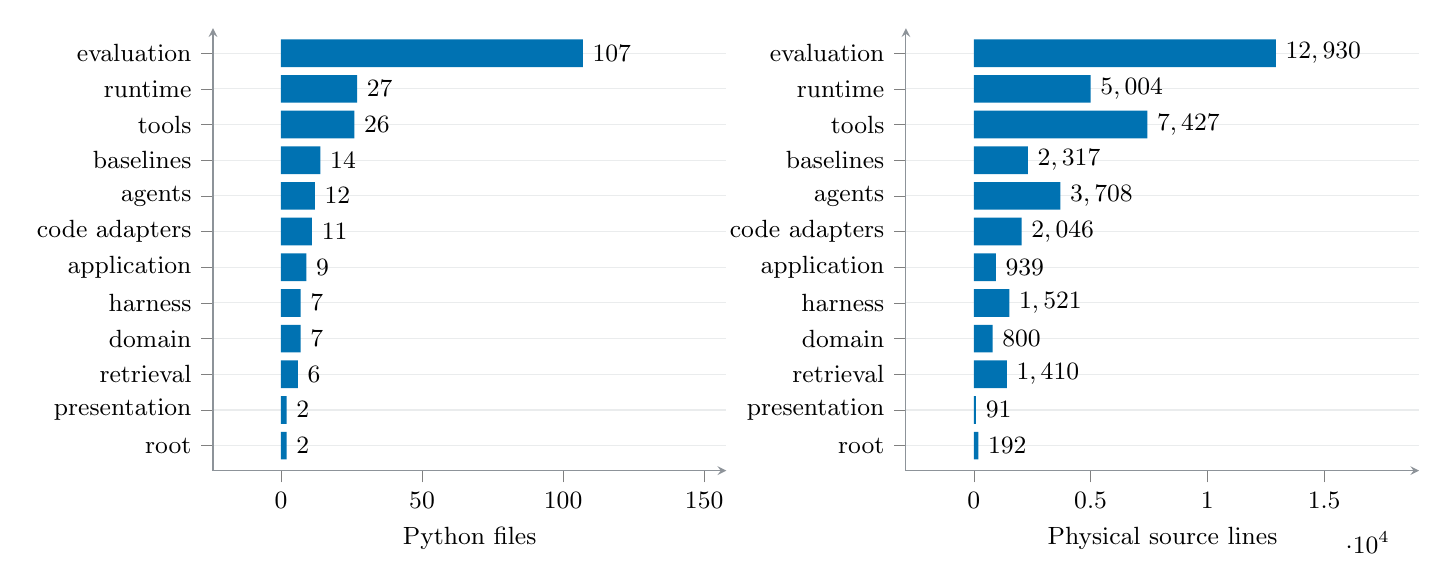
\begin{tikzpicture}
\begin{axis}[at={(0.0cm,0)},anchor=south west,xbar,height=7.2cm,ymin=-.7,ymax=11.7,ytick={0,1,2,3,4,5,6,7,8,9,10,11},yticklabels={root,presentation,retrieval,domain,harness,application,code adapters,agents,baselines,tools,runtime,evaluation},xlabel={Python files},xmin=0,xmax=133.75,nodes near coords,point meta=x]
\addplot[fill=blue,draw=none] coordinates {(2,0) (2,1) (6,2) (7,3) (7,4) (9,5) (11,6) (12,7) (14,8) (26,9) (27,10) (107,11)};
\end{axis}
\begin{axis}[at={(8.8cm,0)},anchor=south west,xbar,height=7.2cm,ymin=-.7,ymax=11.7,ytick={0,1,2,3,4,5,6,7,8,9,10,11},yticklabels={root,presentation,retrieval,domain,harness,application,code adapters,agents,baselines,tools,runtime,evaluation},xlabel={Physical source lines},xmin=0,xmax=16162.5,nodes near coords,point meta=x]
\addplot[fill=blue,draw=none] coordinates {(192,0) (91,1) (1410,2) (800,3) (1521,4) (939,5) (2046,6) (3708,7) (2317,8) (7427,9) (5004,10) (12930,11)};
\end{axis}
\end{tikzpicture}
\end{document}
